\documentclass[tikz,border=8pt]{standalone}
\usepackage{amsmath,amssymb}
\usetikzlibrary{arrows.meta,calc,decorations.markings,decorations.pathmorphing,patterns,shapes.geometric,positioning}

\begin{document}
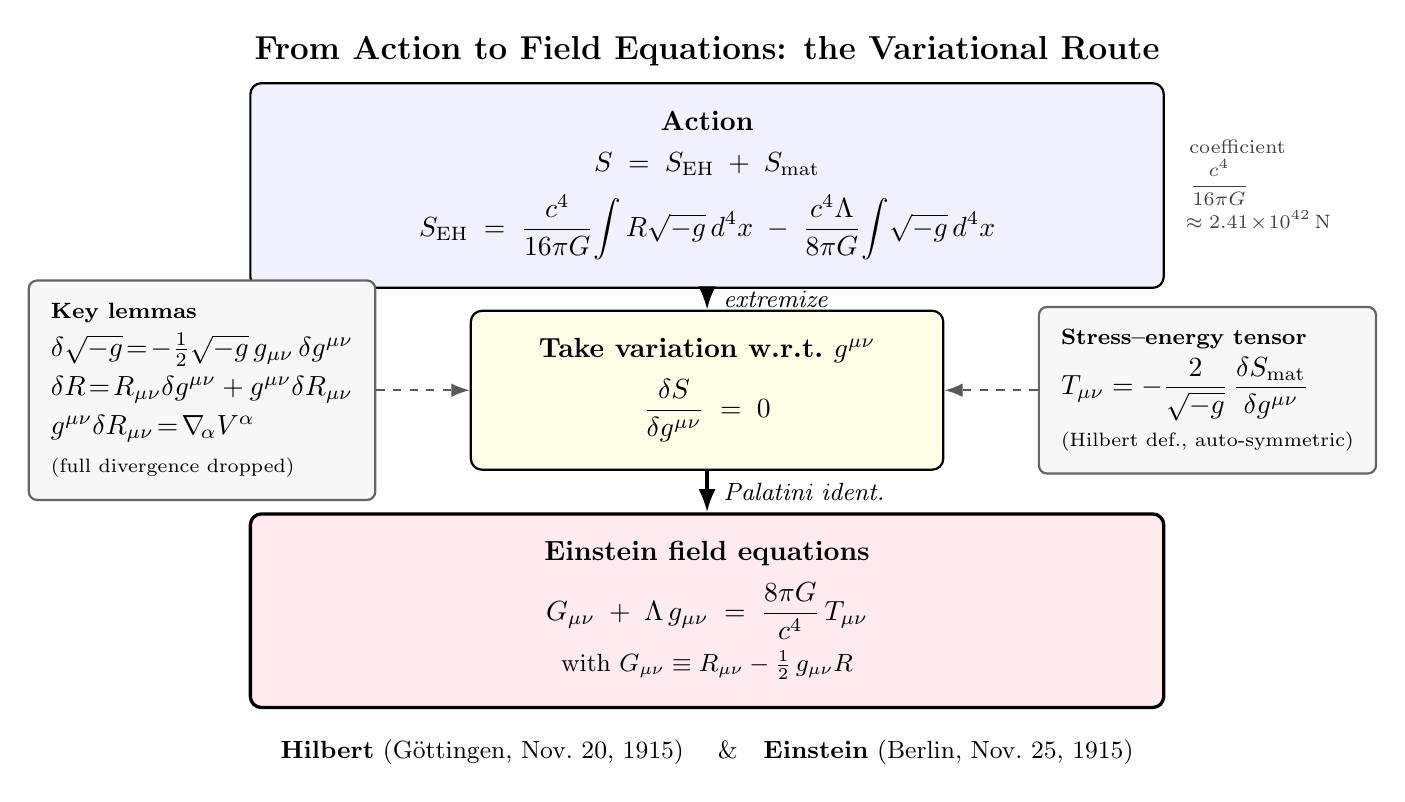
\begin{tikzpicture}[>=Latex,
  topbox/.style={rectangle, draw=black, thick, rounded corners=4pt,
                 fill=blue!6, inner sep=10pt, minimum width=11.6cm, align=center},
  midbox/.style={rectangle, draw=black, thick, rounded corners=4pt,
                 fill=yellow!10, inner sep=10pt, minimum width=6.0cm, align=center},
  botbox/.style={rectangle, draw=black, very thick, rounded corners=4pt,
                 fill=red!8, inner sep=10pt, minimum width=11.6cm, align=center},
  sidebox/.style={rectangle, draw=black!60, thick, rounded corners=3pt,
                  fill=gray!6, inner sep=8pt, align=left}]

  % --- Title at very top ----------------------------------------------------
  \node[font=\large\bfseries, align=center] at (0, 7.7) {%
    From Action to Field Equations: the Variational Route};

  % --- Top: total action ----------------------------------------------------
  \node[topbox] (top) at (0, 6.0) {%
    \textbf{Action} \\[3pt]
    $\displaystyle S \;=\; S_{\rm EH} \;+\; S_{\rm mat}$ \\[6pt]
    $\displaystyle S_{\rm EH} \;=\; \frac{c^{4}}{16\pi G}\!\int R\sqrt{-g}\,d^{4}x
       \;-\; \frac{c^{4}\Lambda}{8\pi G}\!\int\!\sqrt{-g}\,d^{4}x$%
  };

  % --- Middle: variation ----------------------------------------------------
  \node[midbox] (mid) at (0, 3.4) {%
    \textbf{Take variation w.r.t.\ $g^{\mu\nu}$} \\[5pt]
    $\displaystyle \frac{\delta S}{\delta g^{\mu\nu}} \;=\; 0$%
  };

  % --- Bottom: Einstein field equation --------------------------------------
  \node[botbox] (bot) at (0, 0.6) {%
    \textbf{Einstein field equations} \\[5pt]
    $\displaystyle G_{\mu\nu} \;+\; \Lambda\, g_{\mu\nu}
       \;=\; \frac{8\pi G}{c^{4}}\, T_{\mu\nu}$ \\[3pt]
    \small with $G_{\mu\nu} \equiv R_{\mu\nu} - \tfrac{1}{2}\, g_{\mu\nu} R$%
  };

  % --- Connecting arrows top -> mid -> bot ----------------------------------
  \draw[->, very thick] (top.south) -- (mid.north)
    node[midway, right=2pt, font=\small\itshape] {extremize};
  \draw[->, very thick] (mid.south) -- (bot.north)
    node[midway, right=2pt, font=\small\itshape] {Palatini ident.};

  % --- Side note: T_munu definition (right of mid) --------------------------
  \node[sidebox, anchor=west] (sidet) at (4.2, 3.4) {%
    \footnotesize\textbf{Stress--energy tensor}\\[2pt]
    $\displaystyle T_{\mu\nu} = -\frac{2}{\sqrt{-g}}\,
       \frac{\delta S_{\rm mat}}{\delta g^{\mu\nu}}$ \\[3pt]
    \scriptsize (Hilbert def., auto-symmetric)%
  };
  \draw[->, thick, dashed, gray!70!black] (sidet.west) -- (mid.east);

  % --- Side note: ingredient lemmas (left of mid) ---------------------------
  \node[sidebox, anchor=east] (sidel) at (-4.2, 3.4) {%
    \footnotesize\textbf{Key lemmas}\\[2pt]
    $\delta\sqrt{-g}\!=\!-\tfrac{1}{2}\sqrt{-g}\,g_{\mu\nu}\,\delta g^{\mu\nu}$\\[2pt]
    $\delta R \!=\! R_{\mu\nu}\delta g^{\mu\nu} + g^{\mu\nu}\delta R_{\mu\nu}$\\[2pt]
    $g^{\mu\nu}\delta R_{\mu\nu}\!=\!\nabla_{\!\alpha}V^{\alpha}$\\[2pt]
    \scriptsize (full divergence dropped)%
  };
  \draw[->, thick, dashed, gray!70!black] (sidel.east) -- (mid.west);

  % --- History footer (below bottom box) ------------------------------------
  \node[font=\small, align=center] at (0, -1.2) {%
    \textbf{Hilbert} (G\"ottingen, Nov.\ 20, 1915) \quad$\&$\quad
    \textbf{Einstein} (Berlin, Nov.\ 25, 1915)};

  % --- Coefficient annotation right of top box ------------------------------
  \node[anchor=west, font=\scriptsize, align=left, text=black!75] at (6.0, 6.0) {%
    coefficient\\[1pt]
    $\dfrac{c^{4}}{16\pi G}$ \\[1pt]
    $\!\approx 2.41\!\times\!10^{42}\,\mathrm{N}$};

\end{tikzpicture}
\end{document}
